\chapter{Silicon Detectors for High Energy Physics}
\label{chap:silicon}

Pixel and strip detectors realised on high resistivity silicon substrates are nowadays the standard 
choice for high energy physics experiments. 
In this Chapter an introduction to silicon detectors will be given, focusing 
on those aspects that are relevant for the purpose of tracking and vertexing.
Excellent books on the subject exists, like~\cite{Lutz:411172,Sze1981,Wang1989,Krammer}. Here 
some extracts from those will be reported, just to introduce the subject. 
After reviewing the basics  a discussion on radiation damage in silicon 
will follow in Section~\ref{sec:RadDam}.
\section{Semiconductor Basics}

\subsection{Crystals and Energy Bands}

The physics of semiconductor devices is naturally dependent on the physics of semiconductor 
themselves~\cite{Sze1981}. In this brief introduction only crystalline semiconductors will be treated, 
with a particular focus on silicon. Most commonly used semiconductors are crystals with 
diamond (Si and Ge) or zinc blende ({\it e.g.} GaAs) lattice type. In Figure~\ref{fig:diamondLattice} 
a schematic view of the diamond lattice is presented.


\begin{figure}[htbp]
   \centering
   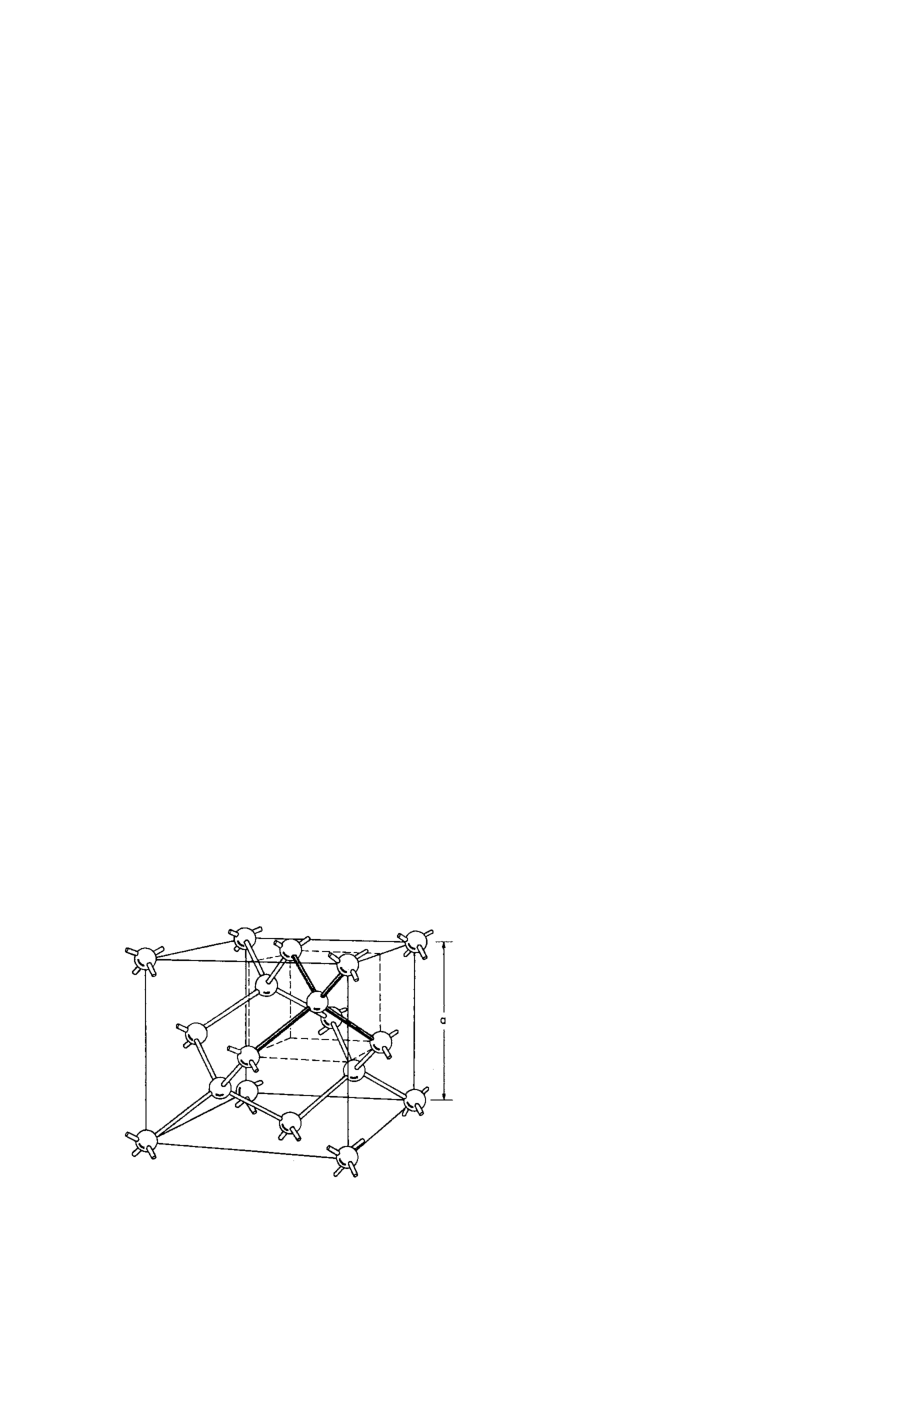
\includegraphics{diamondLattice.pdf} % requires the graphicx package
   \caption{\label{fig:diamondLattice}Diamond (a) and zinc blend (b) lattice. (After~\cite{Lutz:411172})}
\end{figure}

Due to the Pauli exclusion principle, electrons in crystals are organised in energy bands, 
each one containing many closely spaced levels; Figure~\ref{fig:EnergyLevels} helps in picturing 
the situation for diamond lattice. At very large distances each atom has the same two energy levels; 
the energy levels are $N$-fold degenerate ($N$ being the number of atoms), they indeed split 
into $N$ closely spaced levels when the atoms are brought close together. 
For $N\to\infty$, one speaks of energy bands, rather than levels, and these bands broaden, merge 
and split again with even closer spacing~\cite{Lutz:411172}.

\begin{figure}[htbp]
   \centering
   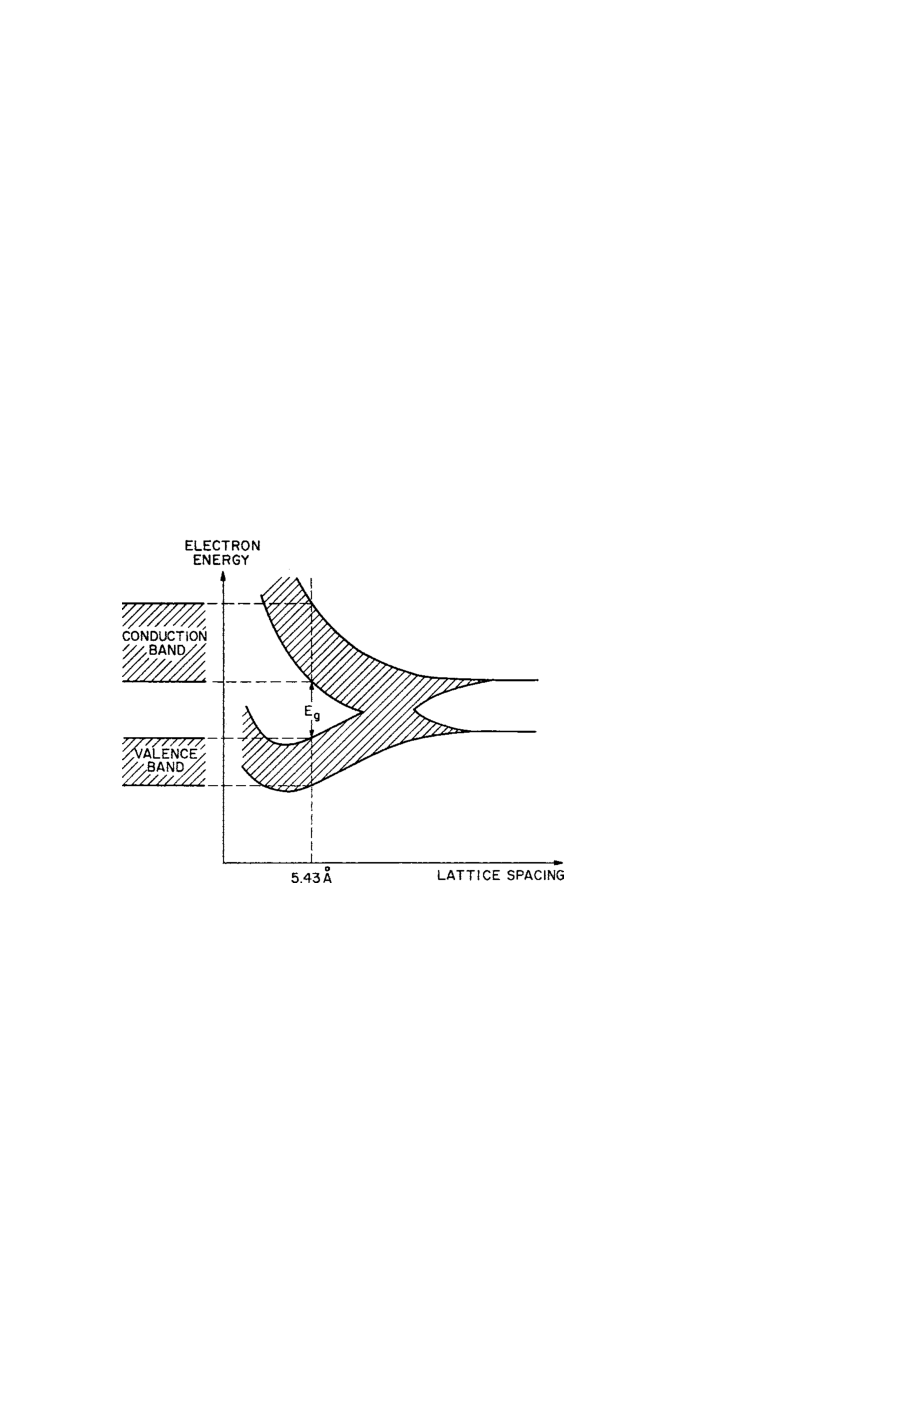
\includegraphics{EnergyLevels.pdf} % requires the graphicx package
   \caption{\label{fig:EnergyLevels}Energy levels of silicon atoms arranged in a diamond structure, as a function of lattice spacing. (After~\cite{Lutz:411172})}
\end{figure}

The spacing corresponding to silicon is indicated in Figure~\ref{fig:EnergyLevels} and corresponds to 
the minimum total energy of the electrons and the lattice, not very far from the minimum energy of
 the electrons in the filled valence band. 
 At low temperature one has a completely filled valence band and an empty conduction band; at room 
 temperature the thermal energy is high enough to lift a few electrons to the conduction band, thus 
 creating a weak conductivity due to free electrons and electrons vacancies, {\it i.e.} holes.
In Figure~\ref{fig:EnergyBandGap} the energy band structures of several materials are reported. 
From that Figure it can be seen that in semiconductors at low temperature one has a completely filled valence band and an empty conduction band; at room 
temperature the thermal energy is high enough to lift a few electrons to the conduction band, thus 
creating a weak conductivity due to free electrons and holes.
 
 \begin{figure}[htbp]
   \centering
   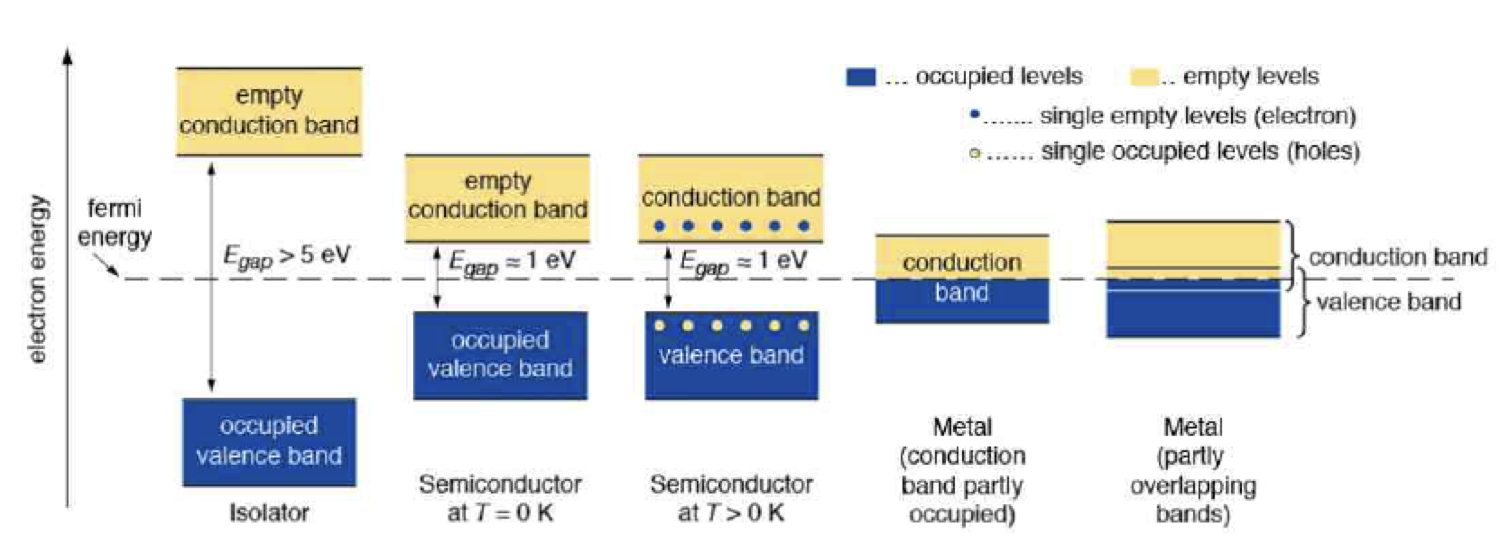
\includegraphics[width=0.8\textwidth]{EnergyBandGap.png} % requires the graphicx package
   \caption{\label{fig:EnergyBandGap}Energy band structure of several materials. For 
   semiconductors the  $T=0$~K and $T>0$~K situations are reported; for metals two 
   possible band configurations are represented (After~\cite{Krammer}).}
\end{figure}


 The structure of an isolator, or insulator, is similar,  except that the band gap is much larger so that 
 the occupation probability of states in the conduction band is zero.   Conductors may either have 
 overlapping valence and conduction bands  or a partially filled conduction band. 
 We can conclude that the main difference between conductors, semiconductors and insulators 
 is the value of the band gap energy $E_g$.
 
 \begin{figure}[htbp]
   \centering
   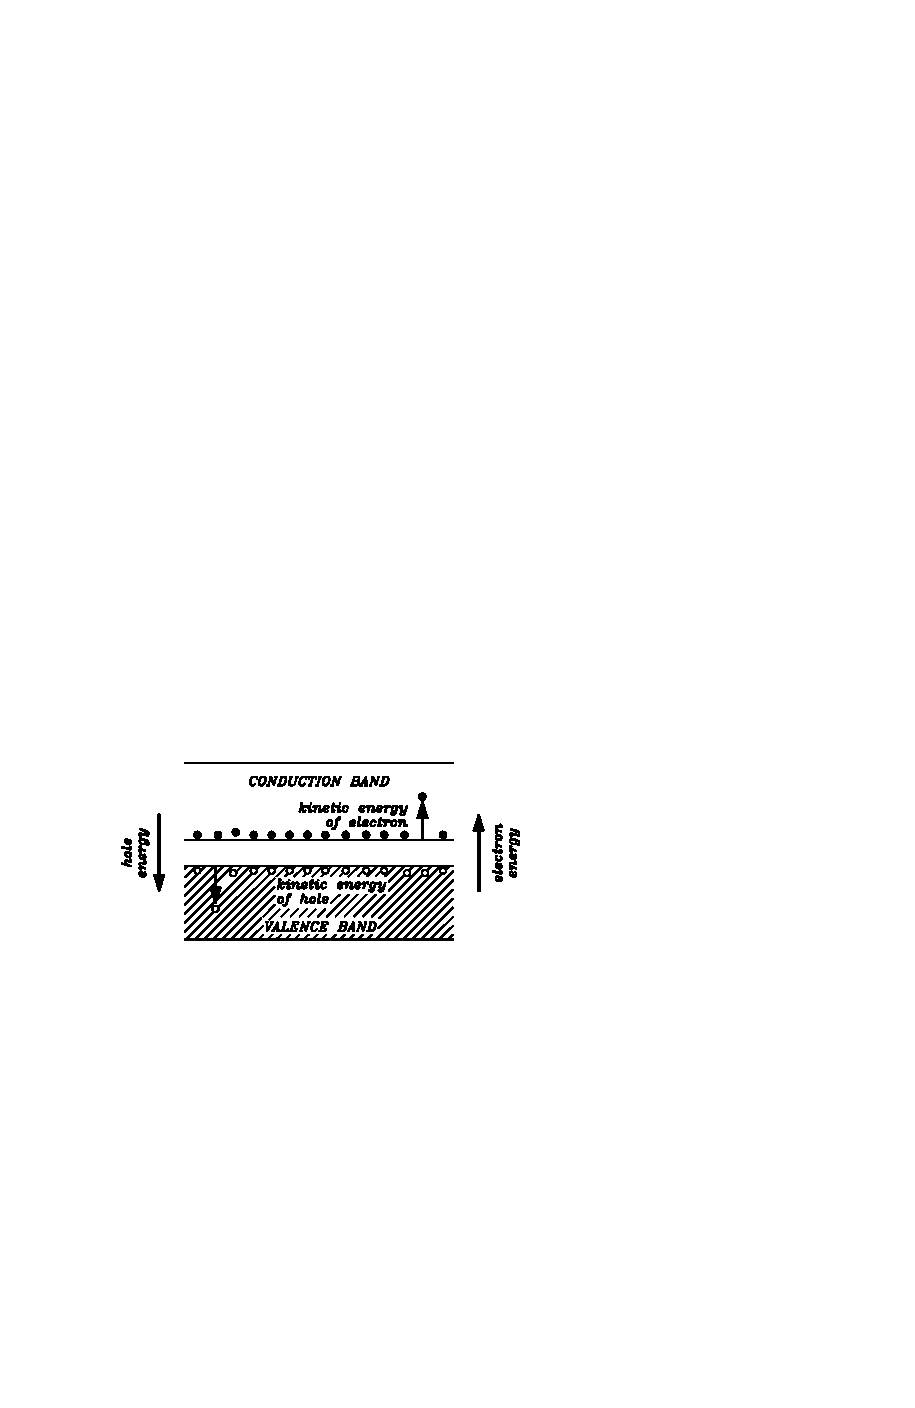
\includegraphics[width=0.55\textwidth]{KinEnergy.pdf} % requires the graphicx package
   \caption{\label{fig:KinEnergy}Potential and kinetic energy in the band 
   representation (After~\cite{Lutz:411172}).}
\end{figure}

Focusing on the dynamics of carriers in crystalline materials, it can be proven that  electrons in the 
conduction band and holes in the valence band are similar to free particles  but with an effective 
mass 
($m_n^*$, $m_p^*$) different from elementary electrons not imbedded in the lattice.
This mass is furthermore dependent on other parameters such as the direction of movement with 
respect to the crystal axis. The kinetic energy of electrons is measured from the lower edge of the 
conduction band upwards, that of the holes downward from the upper edge of the valence band; 
Figure~\ref{fig:KinEnergy} presents the energy diagram for free electrons and holes in lattice.

This simplified picture presents important limitations; in particular it neglects the relative position 
in lattice reciprocal space of the minimum conduction band and the maximum of the valence band. 
If there is no difference among the two positions then the semiconductor is said to have ``direct'' 
bandgap; otherwise it is an indirect semiconductor. Figure~\ref{fig:bandStructures} shows the difference 
between indirect semiconductors, like Silicon and Germanium, and direct ones, like Gallium Arsenide. 


 \begin{figure}[htbp]
   \centering
   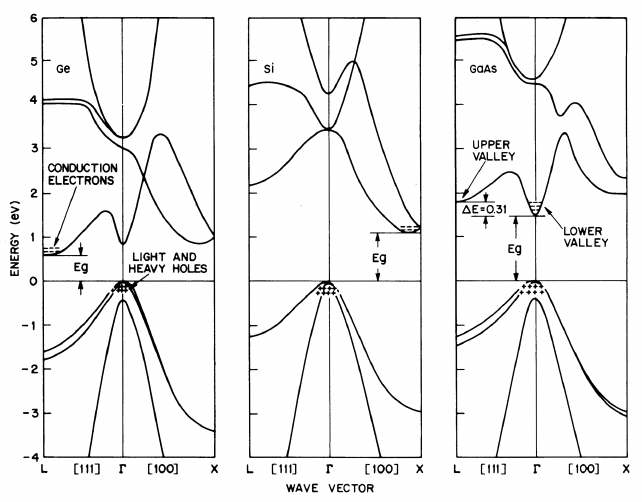
\includegraphics[width=0.55\textwidth]{bandStructures.jpg} % requires the graphicx package
   \caption{\label{fig:bandStructures}Germanium (left), Silicon (center) and Gallium Arsenide (right) band structures. (Bottom) valence bands; (top) conductive bands.}
\end{figure}

For indirect semiconductors, the process of creation or annihilation of an electron-hole pair requires 
not only a quantum of energy, like a photon, but also a net lattice momentum transfer, thanks to 
phonons. In Silicon at room temperature the bandgap energy value is of about $E_g\sim1.12$~eV, 
while the mean ionization energy is $\epsilon~3.6$~eV: the difference is due to the distance in the 
lattice reciprocal space of the edge of conductive and valence band. 

\subsection{Extrinsic Semiconductors and Doping}

Intrinsic semiconductors contain a very limited number of impurities  compared with the number of 
thermally generated electrons and holes. 
Electron states with energy $E$ are occupied following the Fermi-Dirac statistics:
\begin{equation}
F(E)=\dfrac{1}{1+\exp{\Bigg(\dfrac{E-E_F}{kT}}\Bigg)}
\label{eq:FermiDirac}	
\end{equation}
where $E_F$, the Fermi energy, is the energy at which the occupation probability of a (possible) 
state is one half, $k$ is the Boltzmann constant and $T$ is the absolute temperature. 
In Intrinsic semiconductors electrons and holes exist on account of thermal creation of electron-hole 
pairs, so we have:

\begin{equation}
p=n,
\label{eq:n=p}
\end{equation}

{\it i.e.} the concentration of electrons $n$ equals that of holes $p$. 
We will assert the mass action law for semiconductors:
\begin{equation}
np=n_i^2
\label{eq:massLawAction}
\end{equation} 
where $n_i$ is the {\it intrinsic carrier concentration}. The intrinsic carrier concentration depends only 
on the temperature $T$, the effective mass of the carriers $m^*$ 
and the band gap energy 
$E_g$~\cite{Lutz:411172}.


Intrinsic semiconductors are rarely used in semiconductor 
devices since it is extremely difficult to obtain sufficient purity in the material. Moreover, in most cases 
one intentionally alters the property of the material by adding small fractions of specific impurities. 
This procedure is called doping.  Doping is the replacement of a small number of atoms in the lattice by 
atoms of neighbouring columns from the atomic table (with one valence electron more or less compared 
to the basic material). Depending on the type of added material, one obtains n-type 
semiconductors with an excess of electrons in the conduction band or p-types with additional holes in 
the valence band. 

Doping Silicon with an element of the V group (P, As, Sb) leaves a valence electron of dopant atom 
loosely bound; those atoms are identified  
as {\it donor} dopants. The energy level of the donor is just below the edge of the conduction band; 
at room temperature most electrons are raised from the donor dopant to the conduction band.  
The doping with donors  is illustrated in Figure~\ref{fig:nDoping}. A semiconductor doped with 
donors is called a $n-$type semiconductor. There is an imbalance between 
electrons over holes in $n$-type semiconductors; electrons are the majority carriers, while holes the
minority ones. 

 \begin{figure}[htbp]
   \centering
   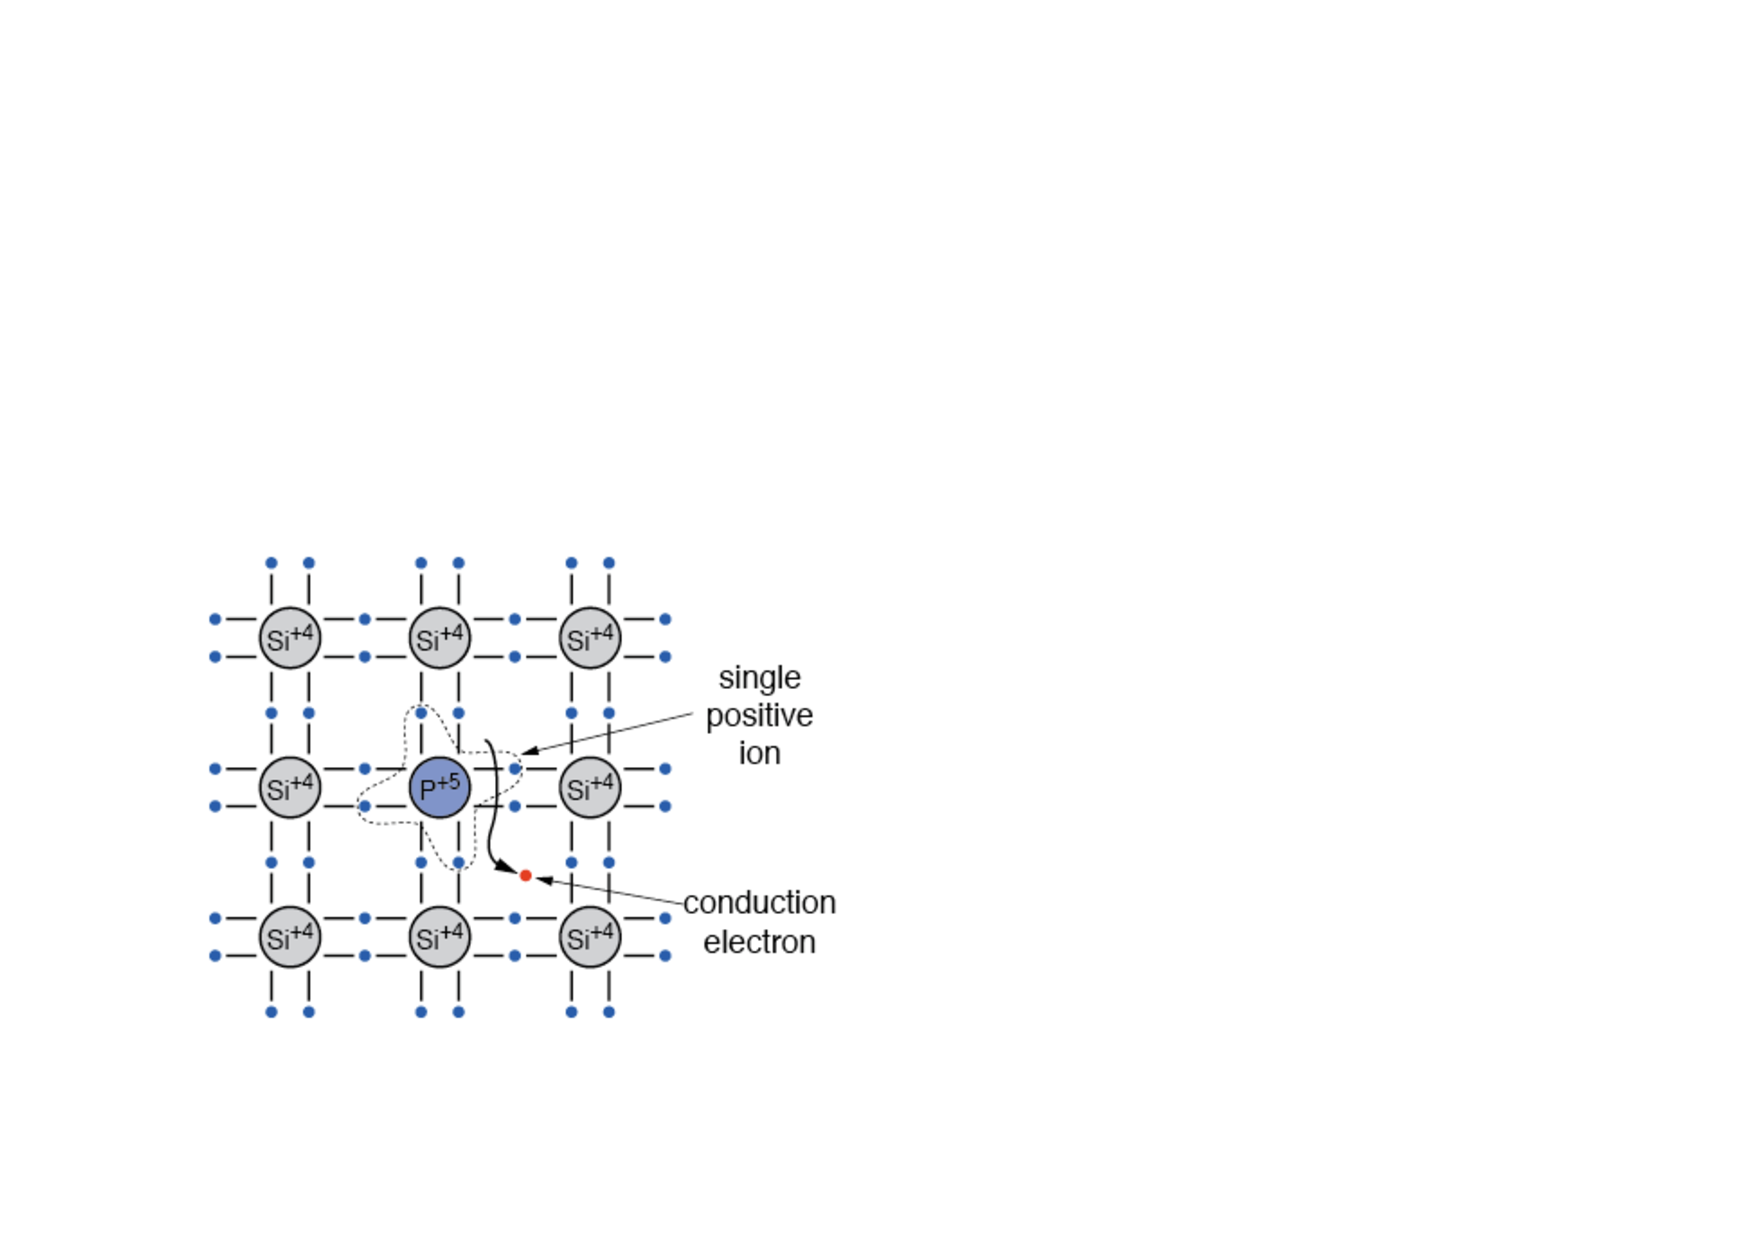
\includegraphics[width=0.45\textwidth]{nDopingBonds.pdf} 
   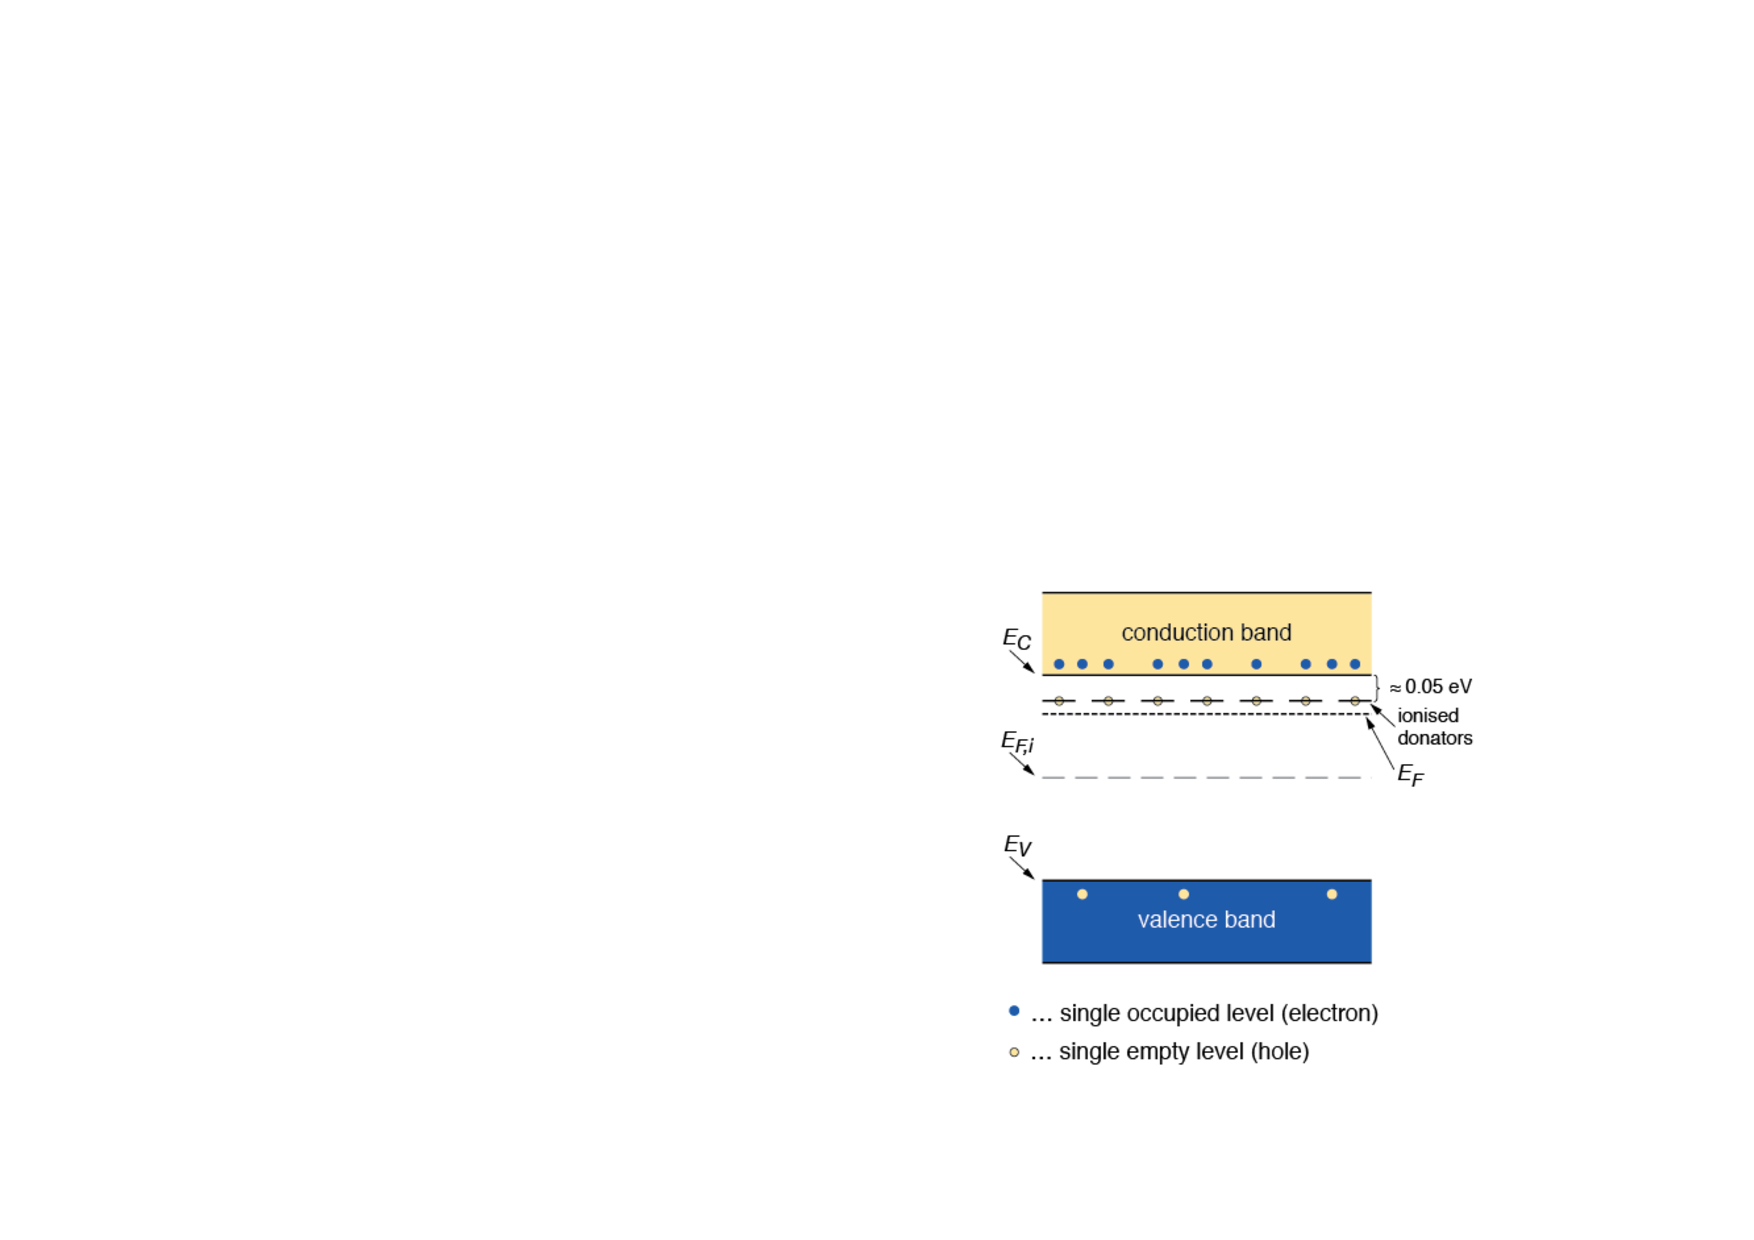
\includegraphics[width=0.35\textwidth]{nDopingBands.pdf} 
   \caption{\label{fig:nDoping}Doping Silicon with donor atoms. (Left) atom bonds with donor dopant; 
   (right) energy bands diagram after donor doping. (After~\cite{Krammer}).}
\end{figure}

Doping Silicon with an element of the III group (B, Al, Ga, In) leaves one valence bond open; 
those atoms are identified  as {\it acceptor} dopants. 
The energy level of the acceptor is just above the edge of the valence band; 
at room temperature most levels are occupied by electrons leaving holes in the valence band.  
The doping with acceptors  is illustrated in Figure~\ref{fig:pDoping}. A semiconductor doped with 
acceptors is called a $p-$type semiconductor. There is an imbalance between 
holes over electrons in $p$-type semiconductors; holes are the majority carriers, while electrons the
minority ones.



 \begin{figure}[htbp]
   \centering
   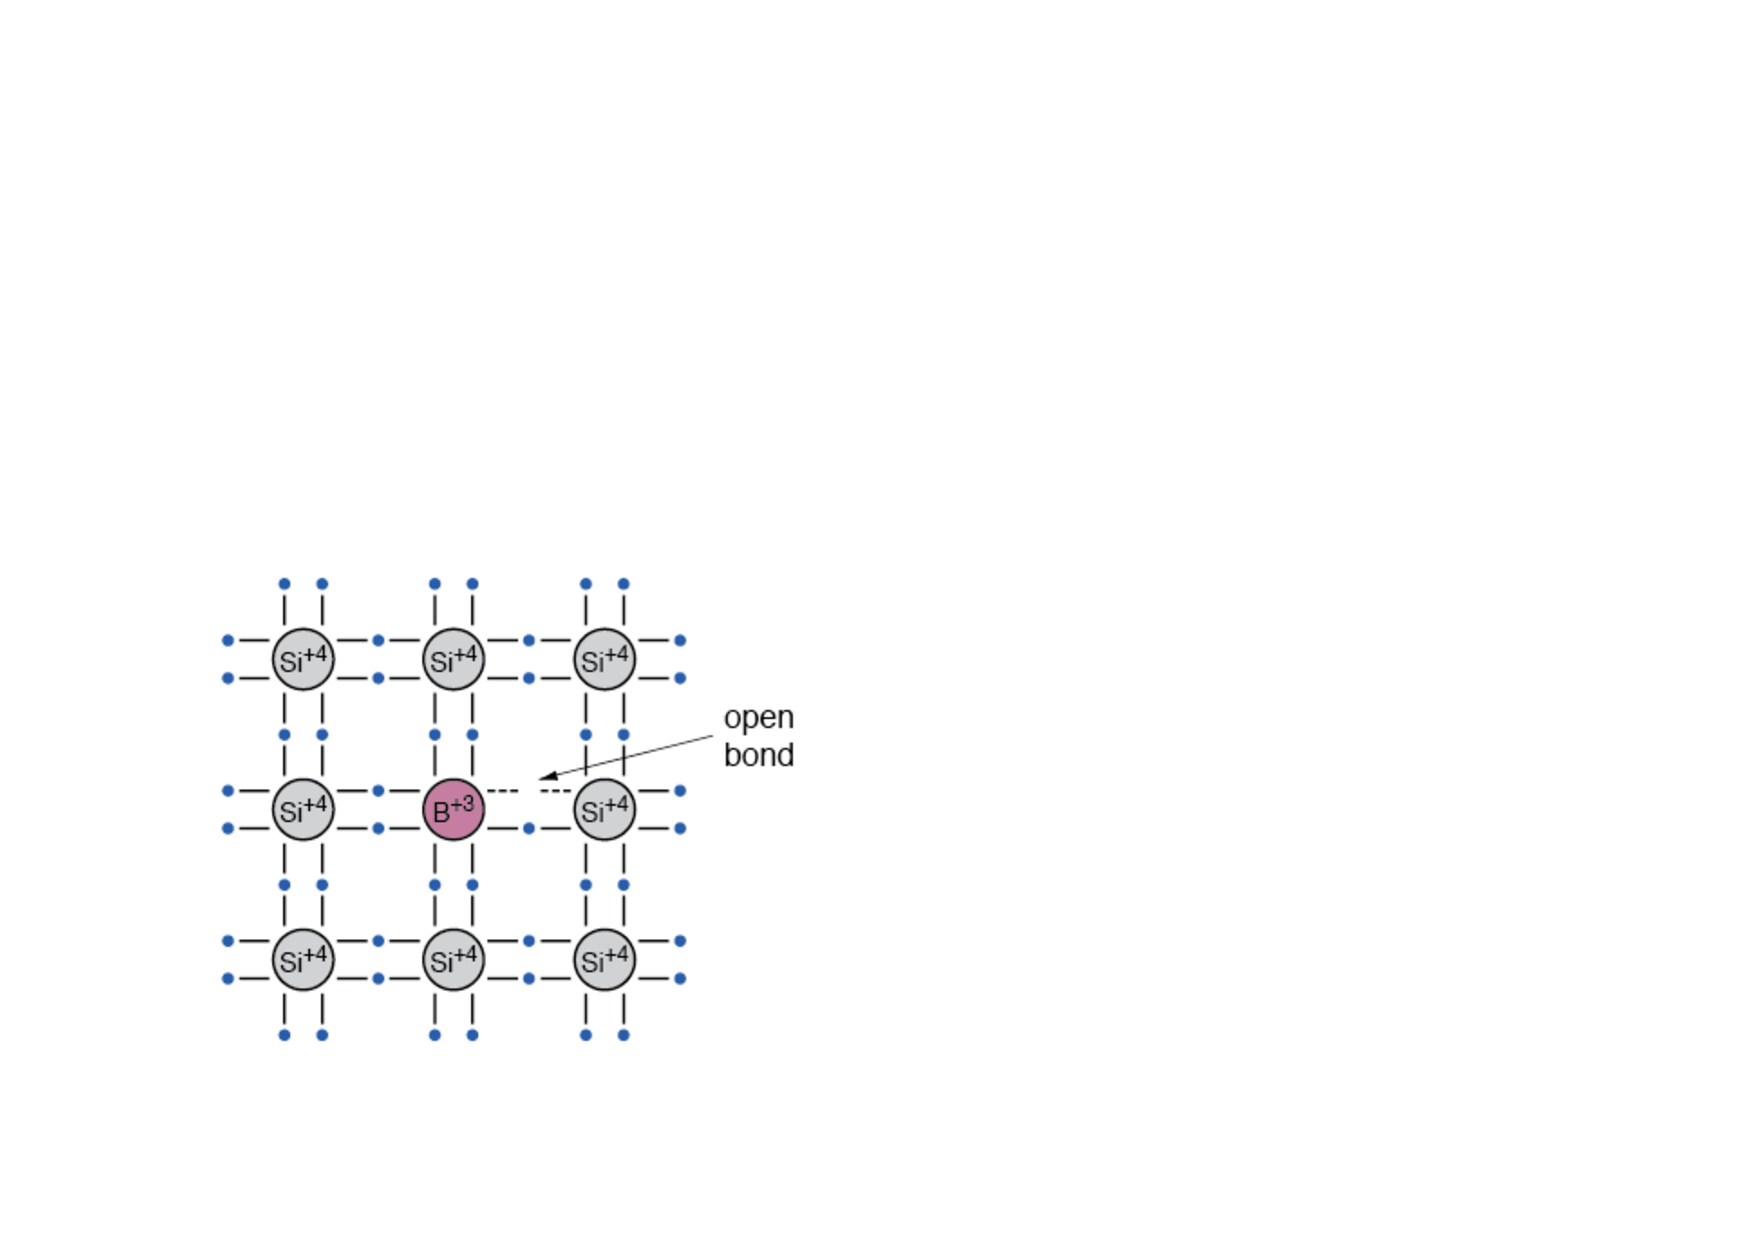
\includegraphics[width=0.45\textwidth]{pDopingBonds.pdf} 
   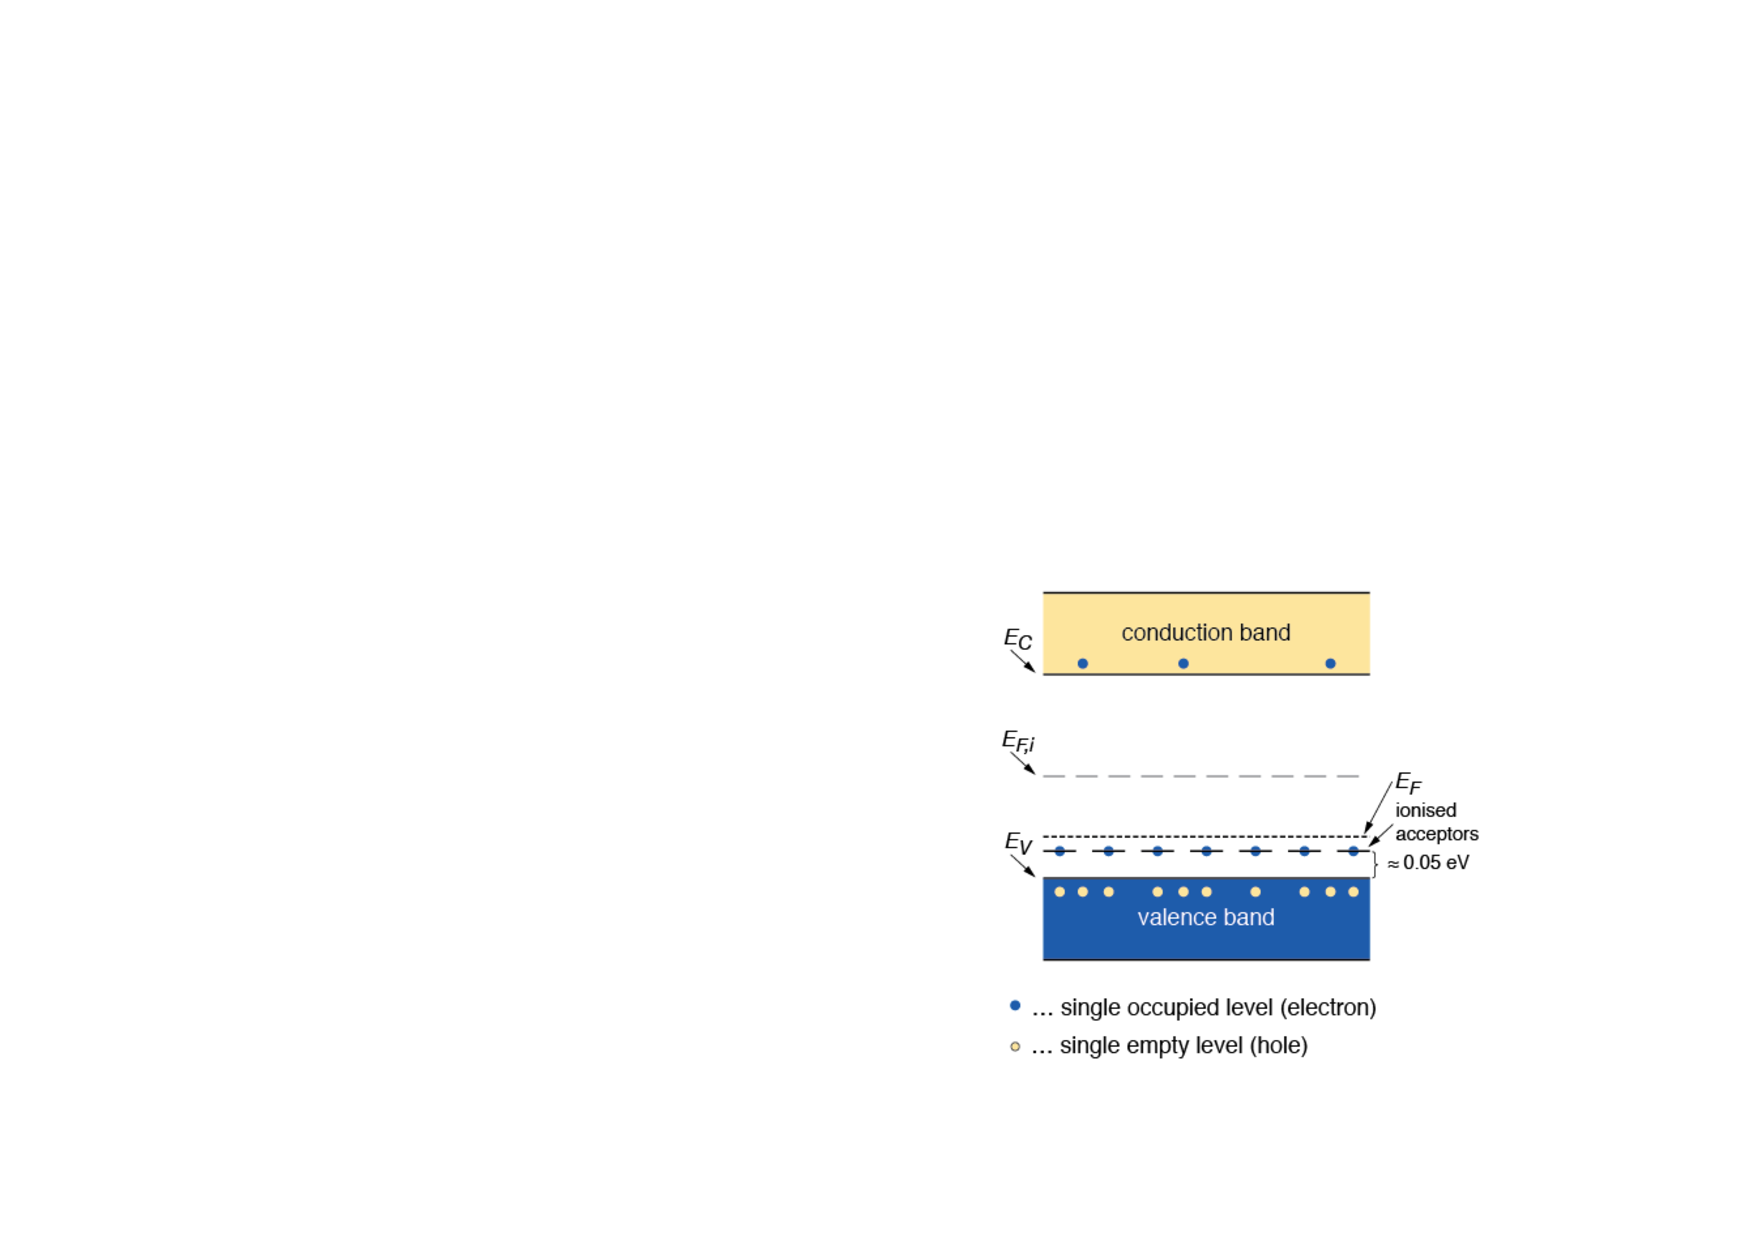
\includegraphics[width=0.35\textwidth]{pDopingBands.pdf} 
   \caption{\label{fig:pDoping}Doping Silicon with acceptor atoms. (Left) atom bonds with acceptor 
   dopant; (right) energy bands diagram after acceptor doping.(After~\cite{Krammer}).}
\end{figure}
In a doped semiconductor the relation $n=p$ doesn't hold, while the mass action law  
(Eqution~\ref{eq:massLawAction}) still does. Semiconductors where $n\neq p$ are called
 {\it extrinsic}.
In a doped semiconductor electrons are merely redistributed among the various energy states, 
but not taken out of or put into the semiconductor itself, the crystal remains electrically neutral. 
The equation that states this charge-neutrality condition reads:

\begin{equation}
n+N_a^-=p+N_d^+,
\label{eq:chargeNeutrality}
\end{equation}

where $N_{a(d)}^{-(+)}$ represent the charge density of ionised acceptors (donors) respectively. 
At room temperature dopants are normally ionised so it is safe to assume that $N_a^-\simeq N_a$ 
and $N_d^+\simeq N_d$, hence $n-p=N_d-N_a$. From charge neutrality and mass action law  
it can be easily shown that for an $n$-type semiconductor the concentration of electrons $n$ is 
equal to that of the donor dopants $N_d$ to a very good level; with the same reasoning in a 
$p$-type semiconductor the concentration of holes $p$ is equal to that of the acceptor 
dopants $N_a$. 

The Fermi level for the intrinsic semiconductor $E_i$ lies very close to the middle of the bandgap.
 When 
impurity atoms are introduced, the Fermi level must adjust itself to preserve charge neutrality. 
We assert that the in an $n$-type semiconductor where the donors concentration is $N_d$ the 
Fermi level at temperature $T$ is:

\begin{equation}
E_F=E_C-kT\ln\Big(\dfrac{N_c}{N_d}\Big)
\label{eq:nEF}
\end{equation}
where $N_c$ is the effective density of states in the conduction band. 
Similarly, in a $p$-type semiconductor where the acceptors concentration is $N_a$ the 
Fermi level at temperature $T$ is:

\begin{equation}
E_F=E_V+kT\ln\Big(\dfrac{N_v}{N_a}\Big)
\label{eq:pEF}
\end{equation}
where $N_v$ is the effective density of states in the valence band. 

The Equations~\ref{eq:nEF}~and~\ref{eq:pEF} can be expressed also as a function of the 
electrons and holes thermal equilibrium concentration $n,p$, and the intrinsic carrier concentration 
$n_i$, to evaluate  the distance of the Fermi level $E_F$ from the intrinsic value $E_i$ 
in an extrinsic semiconductor:

\begin{align}
E_F&=E_i+kT\ln\Big(\dfrac{n}{n_i}\Big)\label{eq:nEini}\\
E_F&=E_i-kT\ln\Big(\dfrac{p}{n_i}\Big)\label{eq:pEini}
\end{align} 




\subsection{Carrier Transport in Semiconductors and Continuity Equations}

So far only semiconductors in equilibrium have been considered. We will now deal with 
semiconductors out of equilibrium through the application of an external voltage or because 
hit by light. These conditions will lead to an inhomogeneous distribution of charge carriers that 
we will describe through the {\it continuity equations}. But before
 getting to the continuity equations let's 
review very briefly the mechanisms of transport of the 
carriers, the drift and the diffusion.

If an electric field is present the charge carriers will be accelerated in between random collisions  
(the typical time between collisions $\tau_c$ is of about 10$^{-12}$~s), 
in a direction determined by the electric field and a net average drift velocity will be obtained, 
equal to:
\begin{align}
\vec{v}_n=-\dfrac{q\tau_c}{m_n}\vec{E}&=-\mu_n\vec{E}\label{eq:nDrift}\\
\vec{v}_p=\dfrac{q\tau_c}{m_p}\vec{E}&=\mu_p\vec{E}\label{eq:pDrift}
\end{align}
$\vec{v}_n$ and $\vec{v}_p$ are the drift velocities.
The parameters $\mu_n,\mu_p$ are the electrons and holes mobilities, respectively. 
For fields small enough the mobilities are constant, while at large fields the carrier velocities 
reach their saturation values $v_{s,n}$ and $v_{s,p}$. Mobilities depend on temperature and 
doping levels too, other than on the electric field.

If we now consider an inhomogeneous distribution of free charge carriers in a semiconductor crystal 
and neglect all effects that are due to electric fields it can be shown that there is a net flow 
of charges to smooth the charge distribution. This effect is called diffusion and it is mathematically 
described by the diffusion equation:
\begin{align}
\vec{F}_n=-D_n\nabla{n}\label{eq:nDiff}\\
\vec{F}_p=-D_p\nabla{p}\label{eq:pDiff}
\end{align}
Here $\vec{F}_{n,p}$ are the fluxes, $D_{n,p}$ the diffusion constants and 
 $n,p$ the carrier concentrations,  of electrons and holes respectively.

Combining the effects of drift and diffusion, one obtains the current densities:
\begin{align}
\vec{J}_n=q\mu_nn\vec{E}+qD_n\nabla{n}\label{eq:nCurrf}\\
\vec{J}_p=q\mu_pp\vec{E}-qD_p\nabla{p}\label{eq:pCurr}
\end{align}

Mobility and diffusion are related to each other by the Einstein equation:

\begin{align}
D_n=\dfrac{kT}{q}\mu_n\label{nEinst}\\
D_p=\dfrac{kT}{q}\mu_p\label{nEinst}
\end{align}

Carriers can recombine and be generated in pairs; we call $G$ the  generation rate per unit of 
volume and $R$ the  recombination rate per unit of volume. 

Now we can write the continuity equations which will describe the change in carrier concentration 
as the result of the drift, diffusion, generation and recombination phenomena:

\begin{align}
\dfrac{\partial n}{\partial t}&=\dfrac{1}{q}\nabla\cdot\vec{J}_n+G_n-R_n\label{eq:nCont}\\
\dfrac{\partial p}{\partial t}&=\dfrac{-1}{q}\nabla\cdot\vec{J}_p+G_p-R_p\label{eq:pCont}
\end{align}

The electric field $\vec{E}$ is linked to the charge distribution $\rho$ by the Poisson's equation:

\begin{equation}
\nabla\cdot\vec{E}=\dfrac{\rho}{\epsilon_{sc}\epsilon_{0}},
\label{eq:Poisson}
\end{equation}
where $\epsilon_{sc}$ is the relative permittivity of the semiconductor.
%\showthe\font

\section{The p-n Junction}

At the interface of an $n$-type and $p$-type semiconductor the difference in the Fermi levels cause 
diffusion 
of surplus carries to the other material until thermal equilibrium is reached. At this point the Fermi 
level 
is equal. The remaining ions create a 
space charge and an electric field stopping further diffusion. 
The stable space charge region is free of charge carries and is called the depletion zone. 
In Figure~\ref{fig:pnJunction} a p-n junction in thermal equilibrium, before and after its parts are 
brought in contact.

\begin{figure}[htbp]
   \centering
   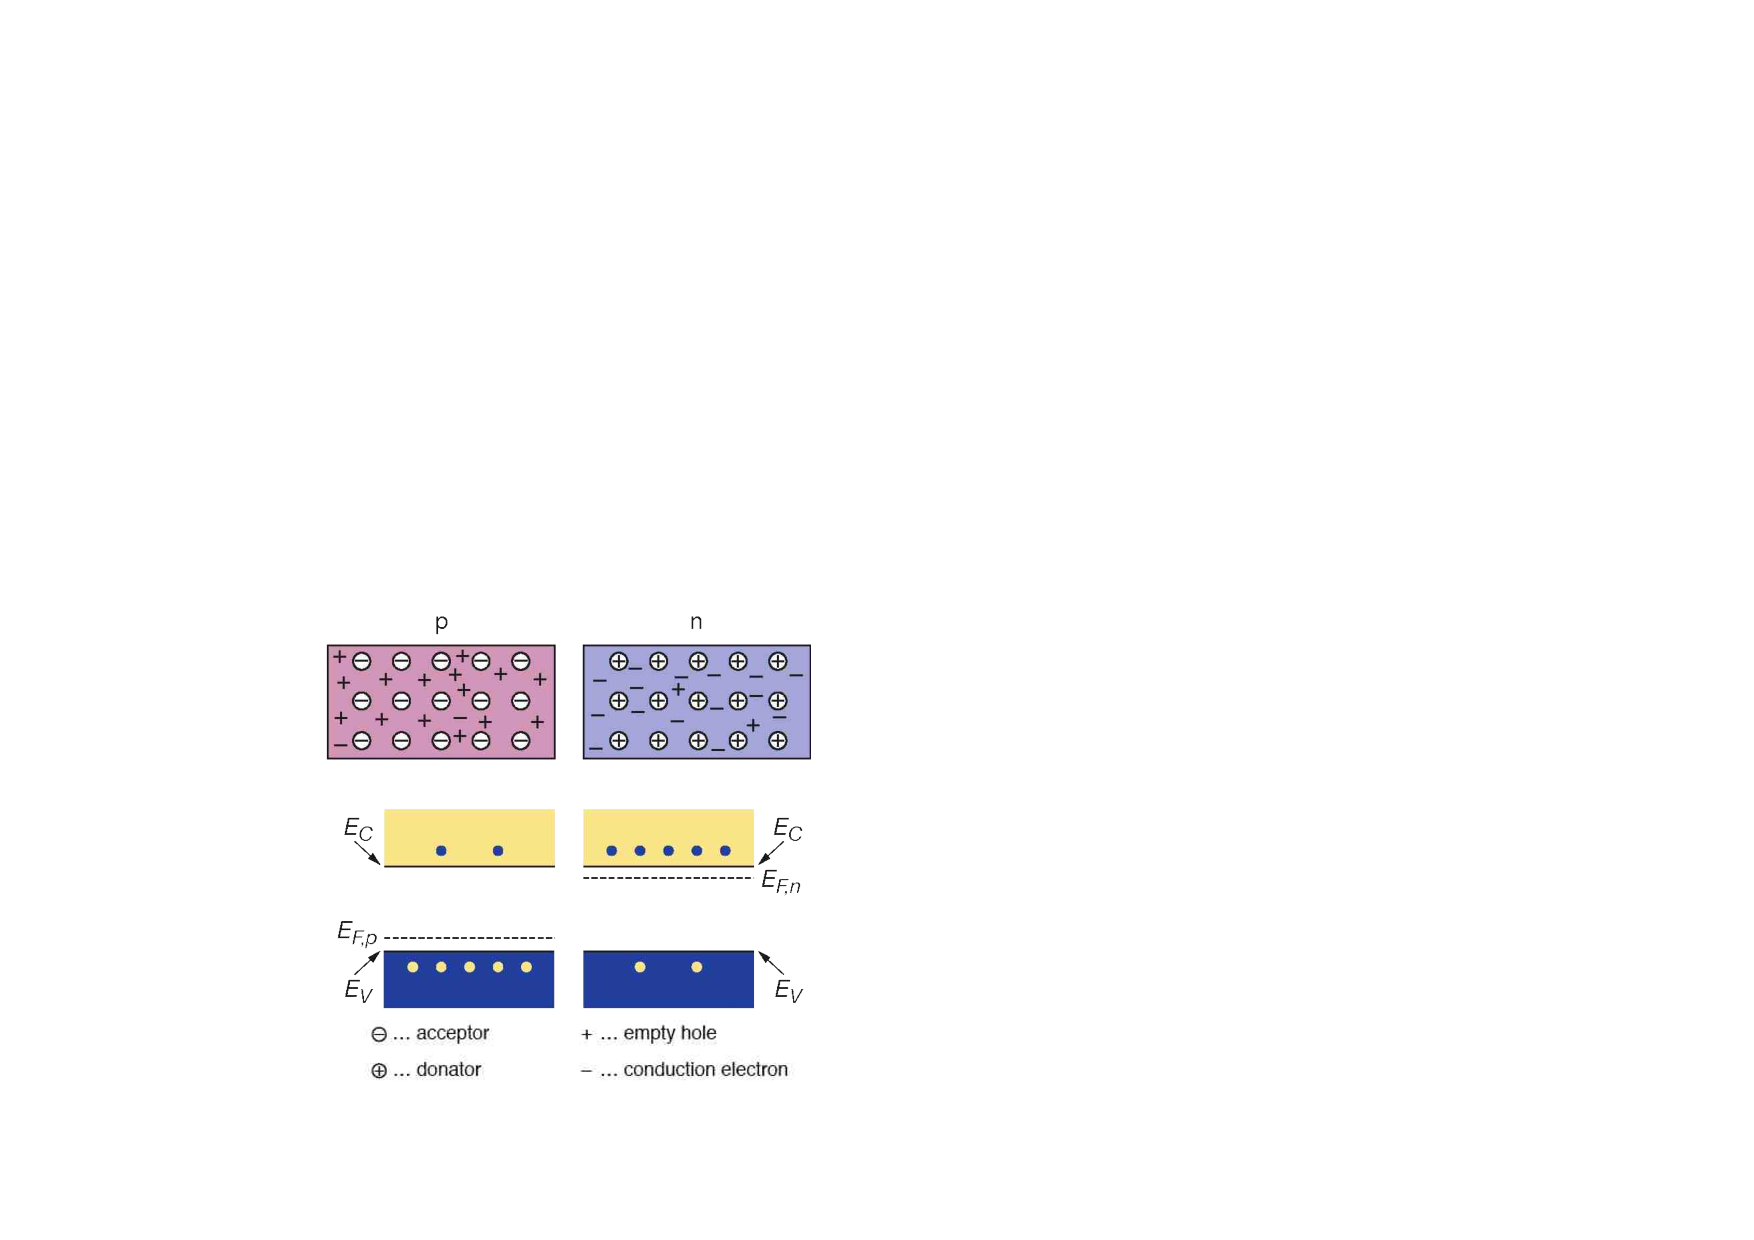
\includegraphics[width=0.45\textwidth]{p_close_to_n.pdf} 
   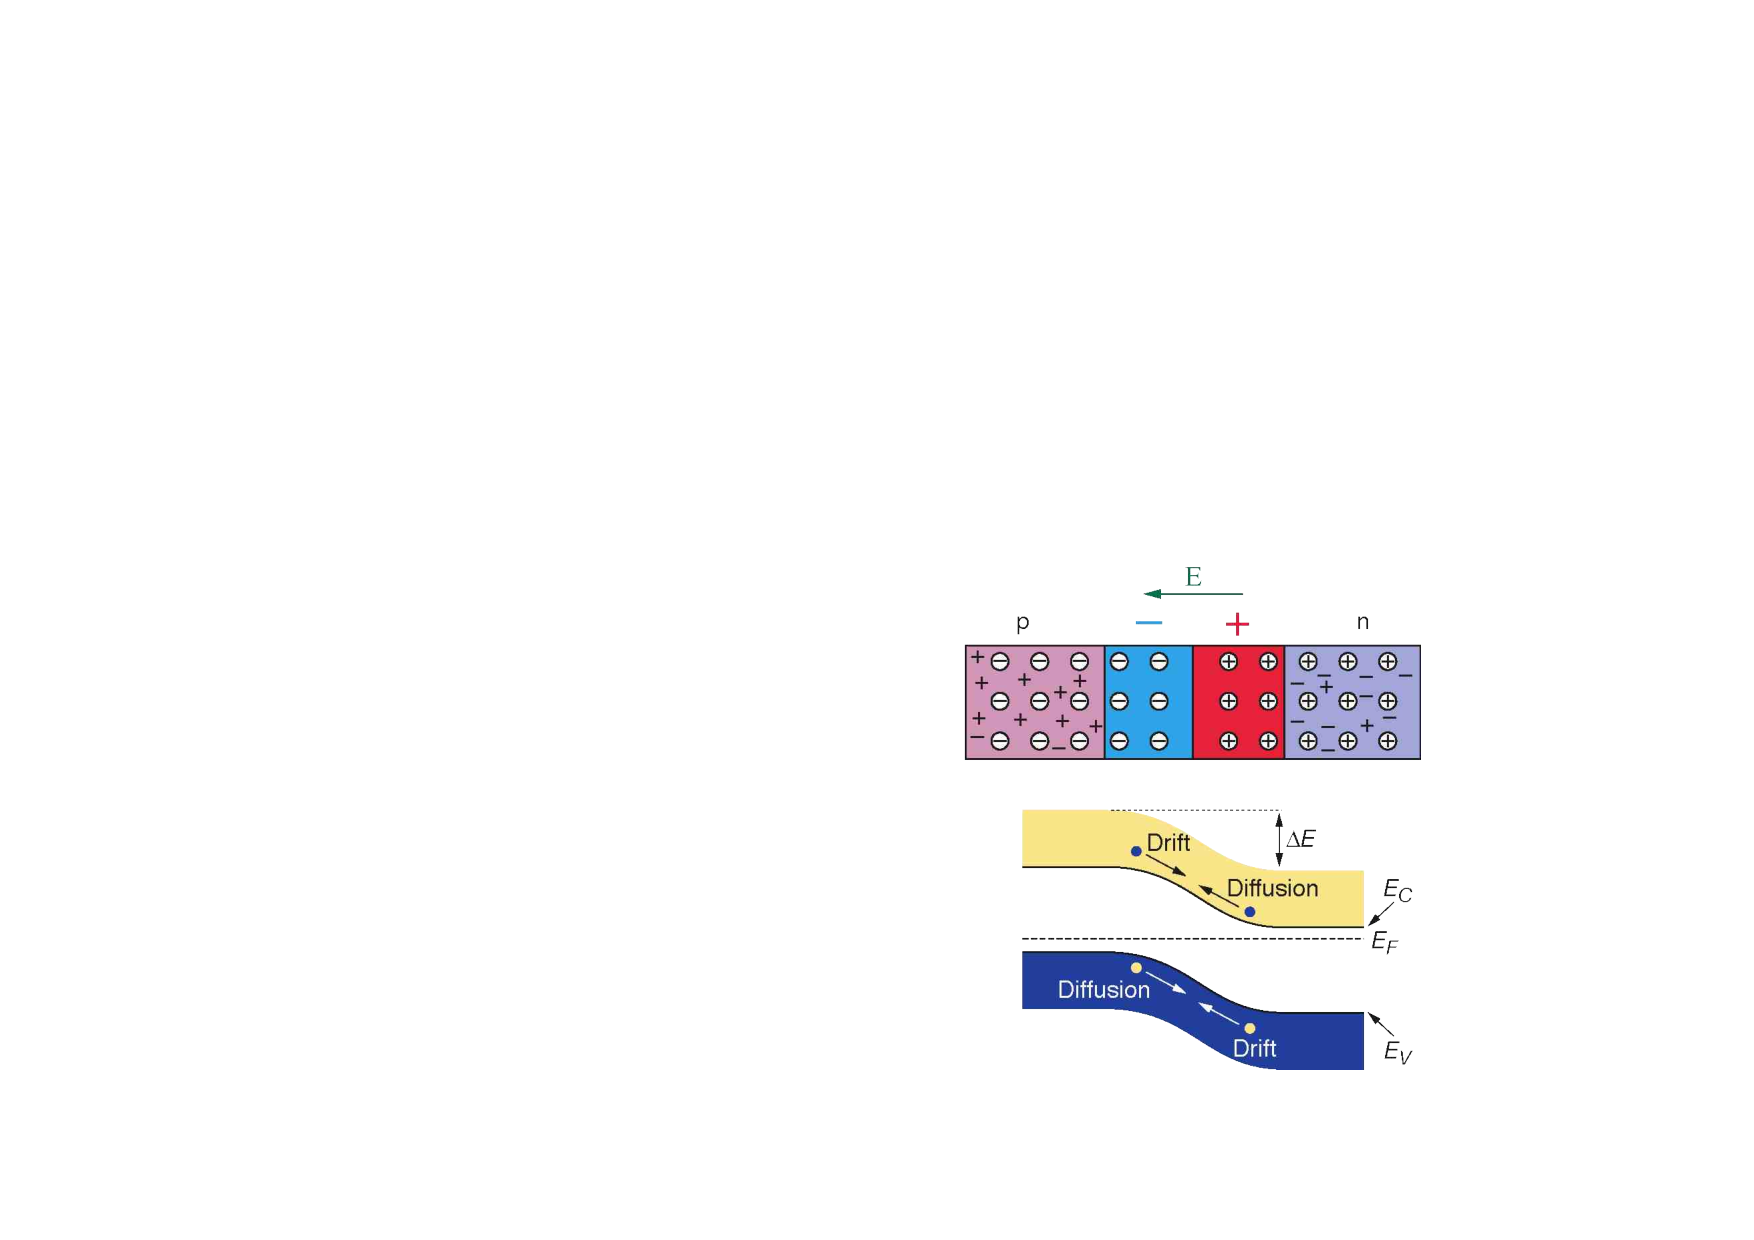
\includegraphics[width=0.45\textwidth]{pn_junction.pdf} 
   \caption{\label{fig:pnJunction}P-n junction formation. (Left) Two oppositely doped semiconductors 
   are compared. (Rigth) The p-n junction is formed. (After~\cite{Krammer}).}
\end{figure}

By applying an external voltage the depletion zone can be shrunk or enlarged. For particle detection 
purpose we are interested in maximising the depletion zone: within it there are virtually no 
free carriers and there is an electric field 
allowing the collection of the free carriers created by the ionising particles. 

By looking at Figure~\ref{fig:pnJunction} it is clear that to deplete more the junction volume 
a potential more positive on the $n$-side than on the $p$-side should be applied; we will refer 
to this polarisation as {\it reverse bias}~voltage.

In the following we will restrict ourselves to abrupt junctions, {\it i.e.} when the doping of both $p$- 
and $n$-type sides of the junction are uniform. Moreover we will consider only the case of 
asymmetric junctions, where one of the two sides is heavily doped, much more doped than the 
other one\footnote{The way in which these junctions are fabricated is beyond the scope of this 
report}. The heavily doped side is usually indicated with a $+$, hence we will talk of 
$p^+-n$ and $n^+-p$ junctions. In Figure~\ref{fig:AAJunction} the charge distribution of 
an abrupt asymmetric $n^+-p$ junction is depicted; the dopant concentration, the 
resulting bulk effective doping concentration and the bulk thickness are indicated too.

\begin{figure}[htbp]
   \centering
   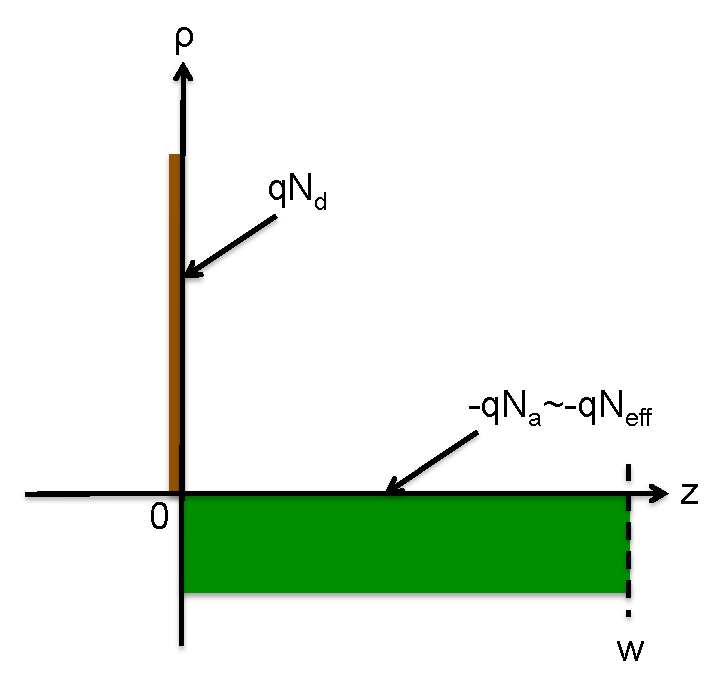
\includegraphics[width=0.45\textwidth]{Abrupt_Junction.pdf} 
      \caption{\label{fig:AAJunction}Charge distribution in an abrupt asymmetric $n^+-p$ junction.}
\end{figure}

To estimate the voltage needed to completely deplete the junction bulk we introduce the concept 
of {\it effective doping concentration} $N_{eff}$:

\begin{equation}
N_{eff} = N_d-N_a
\label{eq:Neff}
\end{equation}
which will reduce to simply $N_d$ for $p^+-n$ junctions and $-N_a$ for $n^+-p$ junctions.
By integrating twice the Poisson's equation over the semiconductor thickness we get 
the voltage needed to achieve the complete depletion of the 
junction volume, the so-called {\it depletion voltage} $V_{depl}$, whose absolute value is equal to:
\begin{equation}
V_{depl}=\dfrac{q|N_{eff}|w^2}{2\epsilon_{sc}\epsilon_0}
\label{eq:vdepl}
\end{equation} 
 where $w$ is the total thickness of the lightly doped semiconductor volume. We stress 
 the fact that the depletion voltage $V_{depl}$ depends linearly on the effective doping 
 concentration $N_{eff}$ and quadratically on the semiconductor volume $w$.

Particle detectors exploiting the $p-n$ junction properties are labelles according to the type 
of the bulk: $p$-type detectors feature a $p$-type bulk, the opposite goes for $n-$type detectors.

If the applied voltage is less than the depletion one we can evaluate the depletion extension 
$d_{depl}$
using again the Poisson's equation. It is instructive to express the result using the {\it resistivity} 
$\varrho$ of the doped semiconductor:

\begin{equation}
\varrho^{-1}=q(N_a\mu_h+N_d\mu_e)\simeq qN_{eff}\mu
\label{eq:resisitivity}
\end{equation}

In Equation~\ref{eq:resisitivity} first the most general expression is presented (under the assumption 
that the carriers concentrations are dominated by the dopants), then the approximated value for an 
abrupt and asymmetric junction is given; $\mu$ is the mobility of the majority carriers.
We can then express the depletion extension $d_{depl}$ as:

\begin{equation}
d_{depl} = \sqrt{2\epsilon_{sc}\epsilon_{0}\mu\varrho|V|}
\label{eq:depletion}
\end{equation}

Comparing Equations~\ref{eq:vdepl}~and~\ref{eq:depletion} a useful relation for under-depleted 
semiconductor bulks can be found:

\begin{equation}
d_{depl} = \sqrt{\dfrac{V}{V_{depl}}}w
\label{eq:dunderdepleted}
\end{equation}
where $V(<V_{depl})$ is the absolute value of the applied bias voltage.

In nowadays trackers for experiments at high energy colliders
 high resistivity materials are used ($\varrho\sim$
 serveral k$\Omega$cm); hence, for thicknesses $w$ of few hundreds of microns depletion voltages of 
 (far) less than 100~V are achieved.

In $p-n$ junctions under reverse bias an electric field is present; if we refer to the case represented 
in Figure~\ref{fig:AAJunction} the electric field distribution at depletion voltage along the bulk is like 
the one shown in Figure~\ref{fig:AAEField}.

\begin{figure}[htbp]
   \centering
   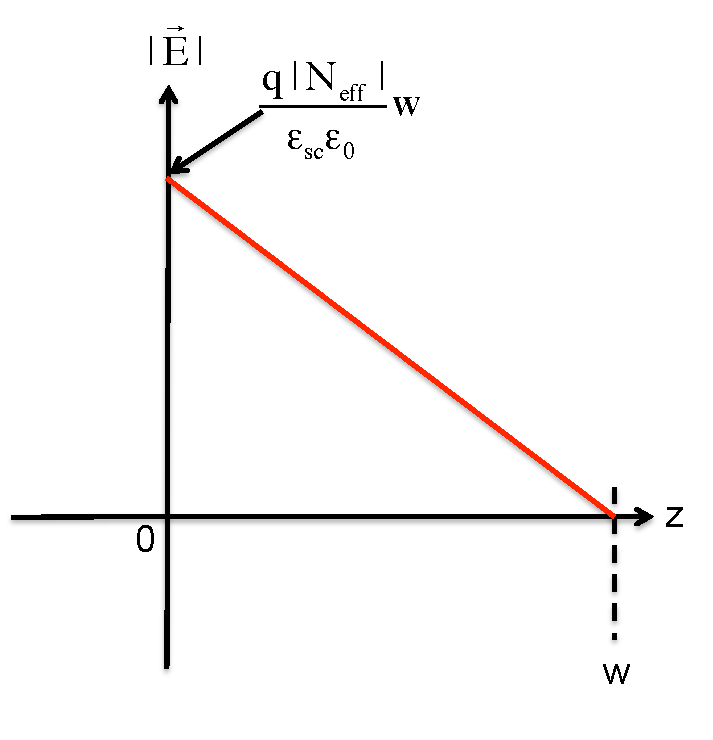
\includegraphics[width=0.45\textwidth]{E_Abrupt_Junction.pdf} 
    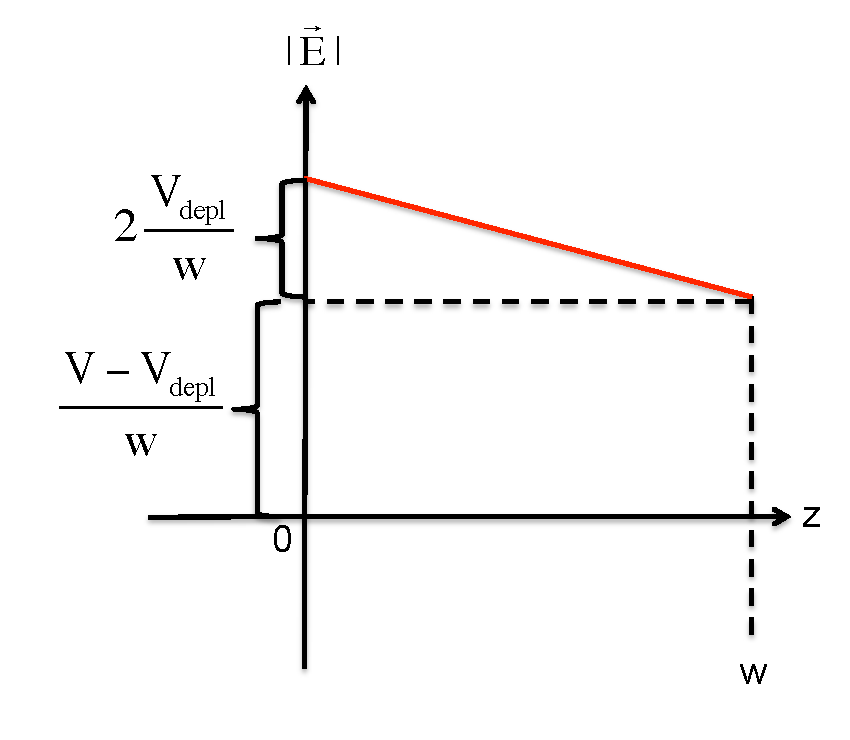
\includegraphics[width=0.45\textwidth]{Overdepleted_E_Abrupt_Junction.pdf}
   \caption{\label{fig:AAEField}Electric field distribution in an abrupt asymmetric $n^+-p$ junction.
   A doping profile like the one reported in Figure~\ref{fig:AAJunction} is assumed. (Left) at 
   depletion voltage; (right) in over depletion.}
\end{figure}
The electric field depends linearly on the bulk depth $z$, with a maximum at the 
junction; the maximum value is proportional to the effective doping concentration.

Still referring to Figure~\ref{fig:AAEField}, if a bias $V$ greater than the depletion 
voltage $V_{depl}$ is applied the electric field will 
have the following dependence on bulk depth $z$:

\begin{equation}
|\vec{E}(z)|=\dfrac{2V_{depl}}{w}\Big(1-\dfrac{z}{w}\Big)+\dfrac{V-V_{depl}}{w}
\label{eq:EFz}
\end{equation}
 The relation between the magnitude of the electric field and the position along the bulk is still 
 linear but now the electric field is non-zero everywhere. The bulk is said to be over-depleted.
 
The depleted region of a $p-n$ junction is out of equilibrium; in particular, since $pn<n_i^2$, in the 
depleted region  the generation process is dominant over recombination. Thermally generated 
electron-hole paris are separated by the electric field.


\section{Why Use Silicon}
Let's know focus only on Silicon. Silicon detectors replaced the  gas based detectors in the tracking systems, since they offer a much
 better position information and an improved energy resolution. The reasons for this are to be found 
in the large density of silicon at room temperature, in the relatively low mean ionisation energy and 
in the possibility of use photolithography to realise charge collecting electrodes. 
These three characteristics allow to have large signals with a small active thickness and 
excellent spatial resolution. Some of the Silicon properties that are relevant for high energy 
physics applications are summarised in Table~\ref{tab:SiProperties}.


% Requires the booktabs if the memoir class is not being used
\begin{table}[htbp]
   \centering
   %\topcaption{Table captions are better up top} % requires the topcapt package
   \begin{tabular}{@{} lcr @{}} % Column formatting, @{} suppresses leading/trailing space
      \toprule
      \multicolumn{3}{c}{Silicon} \\
      \cmidrule(r){1-3} % Partial rule. (r) trims the line a little bit on the right; (l) & (lr) also possible
      Feature    & Value & Comments \\
      \midrule
      Density  $\rho$    & 2.33~g/cm${^3}$ & compact and thin detectors  \\
      Energy bandgap $E_g$ & 1.12~eV & non-cryogenic operation \\
      Mean ionisation energy $\epsilon$ & 3.6~eV & large signals\\
      Radiation length $X_0$      &  9.37~cm & thin detectors to minimize  \\
                                       &                 & multiple scattering \\
      Electron mobility  $\mu_e$     & $\sim$1350 cm$^2$V/s  & fast charge collection \\
      Saturation velocity $v_{sat}$ & $\sim$10$^{7}$ cm/s & fast charge collection \\
      \bottomrule
   \end{tabular}
   \caption{Summary of silicon properties relevant for high energy physics applications~\cite{Lutz:411172}.}
   \label{tab:SiProperties}
\end{table}

Other important characteristics that can explain the success of silicon are its large abundance, 
the possibility of changing its properties by doping, the existence of a natural oxide~\cite{Hartmann2012}.

\section{Silicon Trackers}
\section{Radiation Damage}
\label{sec:RadDam}
